% =====================================================================
%  Research Statement -- Mechanical Engineering (generic version)
%  Lead theme: predictive, trustworthy simulation of fracture, fatigue,
%  and crushing in quasi-brittle solids and granular media
%  Davood Damircheli, Department of Mathematics, Louisiana State University
%  Compile: pdflatex (twice)
%
%  Lines marked  %CHECK  contain claims that should be confirmed before
%  submission (authorship/role on drafts, final numbers, what stays in the
%  submitted crushing paper, etc.).
%  Labels J/S/P/C/M1 match the CV and the other statements; M5--M8 are new
%  labels for mechanics drafts that are not yet on the CV.
% =====================================================================
\documentclass[11pt]{article}
\usepackage[letterpaper,hmargin=1in,vmargin=0.85in]{geometry}
\usepackage[T1]{fontenc}
\usepackage{mathpazo}
\usepackage[scaled=0.95]{helvet}
\usepackage{microtype}
\usepackage{amsmath,amssymb}
\usepackage{xcolor}
\usepackage{enumitem}
\usepackage{titlesec}
\usepackage{tikz}
\usetikzlibrary{positioning,arrows.meta,shapes.misc}
\usepackage[hidelinks]{hyperref}

\definecolor{accent}{RGB}{25,70,125}
\definecolor{soft}{RGB}{235,241,248}

\titleformat{\section}{\normalfont\large\bfseries\color{accent}}{\thesection.}{0.5em}{}
\titlespacing*{\section}{0pt}{9pt}{3pt}
\titleformat{\paragraph}[runin]{\normalfont\bfseries}{}{0pt}{}[.]
\titlespacing*{\paragraph}{0pt}{4pt}{0.6em}
\setlist{nosep,leftmargin=1.3em,topsep=2pt}
\setlength{\parskip}{3pt}
\setlength{\parindent}{0pt}

\renewcommand{\ttdefault}{pcr}
\newcommand{\rc}[1]{\textcolor{accent}{[#1]}}

\begin{document}

% ------------------------------------------------------------- header
\begin{center}
{\LARGE\bfseries Research Statement}\\[3pt]
{\large Davood Damircheli}\\[1pt]
{\small Department of Mathematics, Louisiana State University\\
\href{mailto:ddamircheli@lsu.edu}{ddamircheli@lsu.edu} \;$\cdot$\;
\href{https://davooddamircheli.github.io}{\nolinkurl{davooddamircheli.github.io}} \;$\cdot$\;
\href{https://github.com/DavoodDamircheli}{\nolinkurl{github.com/DavoodDamircheli}}}
\end{center}
\vspace{-4pt}

% ------------------------------------------------------------- overview
\section*{Overview}

Concrete, rock, ceramics, glass, and the crushable grains that make up sand and
other granular media all fail the same way: cracks nucleate, grow, branch, and
eventually break the material into fragments. Predicting this process matters
for protective structures, civil and geotechnical infrastructure, mining and
other energy-intensive comminution, and the design of engineered particulate
materials. It is also where standard simulation tools are weakest. Cohesive-zone
and continuum-damage models need crack paths or failure criteria specified in
advance, phase-field models add a second evolution equation, and the
discrete-element method treats grains as rigid bodies that cannot break.

My research develops \textbf{computational solid mechanics in which fracture,
crushing, and fatigue emerge from the constitutive law itself}, and gives these
models the guarantees an engineer needs to rely on them. I work on three
connected thrusts:
\begin{enumerate}[label=(\roman*),leftmargin=2.2em]
\item \textbf{Fracture models that are well-posed and validated}: nonlocal
      (peridynamic) constitutive laws for quasi-brittle fracture, fatigue, and
      damage--plasticity, checked against experiments with a small set of measurable parameters;
\item \textbf{Grain-scale simulation of crushable granular media}: a 3D
      framework in which every grain is a fracturing body, run on up to
      1{,}600 cores to connect grain shape and breakage to bulk response;
\item \textbf{Simulation tools engineers can trust}: proofs that the
      simulated dynamics are well-defined, stable solvers for contact-type
      constraints, and certified error bounds for machine-learned surrogates.
\end{enumerate}
I was trained on both the engineering and the mathematical side: a Ph.D.\ in
Computational Engineering from Mississippi State's Bagley College of
Engineering (advisor S.~Bhushan, Mechanical Engineering), where my dissertation
developed stable methods for variational inequalities in computational mechanics,
and a Ph.D.\ in Applied Mathematics. As a postdoctoral researcher in Robert
Lipton's group at LSU I have worked on two DoD MURI programs:
\emph{Predicting and Controlling the Response of Particulate Systems through
Grain Scale Engineering} (ARO) and \emph{Complexity, Nonlocality, and
Uncertainty in Heterogeneous Solids}. I present this work at the main
mechanics meetings (USNCCM, USNCTAM, EMI).

\begin{center}
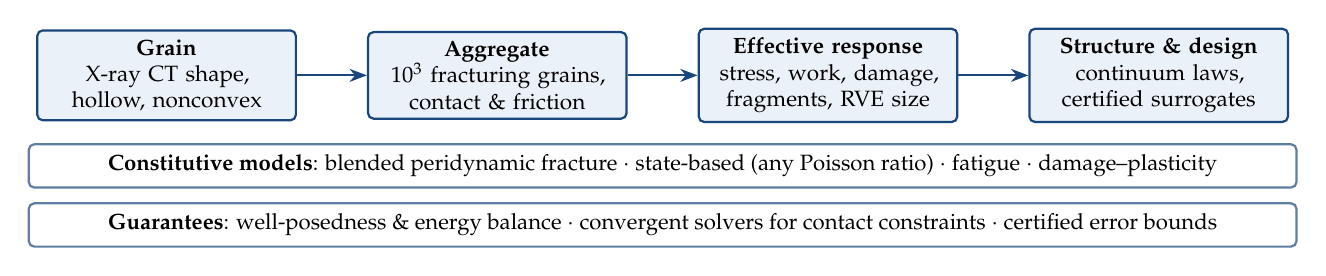
\begin{tikzpicture}[
  font=\footnotesize,
  sc/.style={rectangle, rounded corners=2pt, draw=accent, fill=soft, thick, minimum height=10mm, text width=3.05cm, align=center},
  base/.style={rectangle, rounded corners=2pt, draw=accent!70, fill=white, thick, minimum height=5.5mm, align=center},
  arr/.style={-{Stealth[length=2.2mm]}, accent, thick}]
  \node[sc] (g) at (0,0) {\textbf{Grain}\\X-ray CT shape,\\hollow, nonconvex};
  \node[sc] (a) at (4.2,0) {\textbf{Aggregate}\\$10^3$ fracturing grains,\\contact \& friction};
  \node[sc] (e) at (8.4,0) {\textbf{Effective response}\\stress, work, damage,\\fragments, RVE size};
  \node[sc] (s) at (12.6,0) {\textbf{Structure \& design}\\continuum laws,\\certified surrogates};
  \draw[arr] (g) -- (a); \draw[arr] (a) -- (e); \draw[arr] (e) -- (s);
  \node[base, minimum width=16.1cm] (m) at (6.3,-1.15)
     {\textbf{Constitutive models}: blended peridynamic fracture $\cdot$ state-based (any Poisson ratio) $\cdot$ fatigue $\cdot$ damage--plasticity};
  \node[base, minimum width=16.1cm] (t) at (6.3,-1.9)
     {\textbf{Guarantees}: well-posedness \& energy balance $\cdot$ convergent solvers for contact constraints $\cdot$ certified error bounds};
\end{tikzpicture}
\end{center}
\vspace{-10pt}

% ------------------------------------------------------------- theme 1
\section{Fracture models that are well-posed and validated}

\paragraph{The blended model for quasi-brittle fracture}
With S.~Coskun and R.~Lipton \rc{J3, \emph{J.\ Mech.\ Phys.\ Solids} 2025} we
introduced a model that combines a nonlocal peridynamic force law with a
\emph{two-point phase field}. The phase field is an algebraic function of each
bond's strain history, so damage needs no extra diffusion equation and the
displacement remains the only unknown. Only three material constants are
needed beyond elasticity, all measurable in standard tests: Young's modulus,
tensile strength, and fracture energy. My contribution centered on the
mathematical analysis. The displacement and damage fields are the unique
solution of a single momentum balance. Energy balance with nonnegative
dissipation follows from the equation of motion instead of being imposed. For
flat cracks the dissipated energy equals the Griffith energy
$\mathcal G_c\,\mathcal H^{d-1}(\text{crack})$, independently of the nonlocal
horizon.

The model reproduces monotonic and cyclic load--CMOD curves of three-point
bending tests on high-strength concrete, mixed-mode crack paths in notched
beams, cracking of L-shaped panels, and dynamic crack branching in glass, where
the crack-tip speed stays below $0.6\,c_R$ and the branching time agrees with
phase-field results. It also captures the \textbf{structural size effect}. With
a single set of constants and no size-dependent strength rule, it predicts the
nominal strength of concrete beams 80, 160, and 320\,mm deep; a strength-based
criterion overestimates the two smaller beams by 43\% and 26\%.

\paragraph{Beyond bond-based limits: state-based, plastic, and fatigue damage
(in progress)} %CHECK role on these drafts
The validation exposed two physical gaps that my current work addresses. First,
bond-based peridynamics fixes Poisson's ratio, and its unloading is purely
elastic, so the simulated cyclic curves return to the origin while the
experimental ones do not. A state-based blended model \rc{M7} allows any
Poisson ratio $\nu\in(-1,\tfrac12)$ and introduces separate volumetric and
deviatoric damage channels (mode~I and mode~II). It also adds damage--plasticity
through unloading ratios that leave residual strain, and comes with existence,
uniqueness, and power-balance theorems. Second, a damage law driven by maximum
strain cannot produce fatigue, because cycling below the monotonic threshold
never causes damage. In \rc{M8} a bond-wise \emph{strain-path functional}
accumulates damage only above an endurance threshold. Fatigue then requires
three new parameters, each with a calibration recipe from CMOD hysteresis and
$S$--$N$ data, and the model stays well-posed with nonnegative monotone,
fatigue, and plastic dissipation. Scaling arguments show that $S$--$N$ curves
with an endurance limit and Paris-type crack growth follow from the
constitutive law rather than being fitted.

% ------------------------------------------------------------- theme 2
\section{Crushing and comminution of 3D granular aggregates}

\paragraph{A framework in which grains break}
With D.~Bhattacharya and R.~Lipton \rc{S5} I developed \texttt{PeriGrain3D}, a
3D framework in which every grain of an aggregate is a fracturing peridynamic
body. %CHECK: "I developed the 3D implementation" -- repository is under your GitHub
Grains interact through nonlocal repulsion, Coulomb friction (regularized so
that no surface normals are needed), and contact damping. Fragments of the same
grain interact through self-contact once their bonds have broken, and rigid
walls act through closed-form spherical-cap formulas, so the walls need no
mesh. Nonconvex and hollow grains are built by filtering the reference bond
graph. Crushing, comminution, and fragment interaction then emerge from the
dynamics, with no crack tracking. The framework is verified against Hertz
contact, where it is closer to the analytical force than a published
state-based result, and against the Kalthoff--Winkler impact experiment, where
it reproduces the ${\approx}68^\circ$ crack angle. A compaction study of
125-grain aggregates (0.4--0.5 million material points, up to 12.9 million
bonds) shows how shape controls strength. Nonconvex ``jacks'' rearrange by
rotation and have the lowest bulk strength, and hollow shells are weaker than
solid spheres because fragments fill their internal voids. At large compaction,
strength is governed by volume fraction.

\paragraph{Large-scale simulation and representative specimen size}
To make these simulations useful for continuum modeling, I scaled them to
aggregates of 400--1{,}000 grains, both X-ray-CT-reconstructed sand and hollow
spheres, with about 1.3 million material points. Production runs used up to
1{,}600 cores of LSU's SuperMIC cluster, at 42--56 thousand core-hours each.
%CHECK: keep only if the CT/HPC material stays in S5 or appears in M5
In a companion study \rc{M5} we use the simulator as a computational
laboratory. We define finite-size errors for axial stress, absorbed work,
damage, and fragment statistics (fragments are the connected components of the
intact bond graph), and from them an \emph{accuracy--cost map}: the cheapest
specimen that meets a prescribed tolerance for each quantity of interest. The
study is designed to show that bulk stress and grain-scale damage converge at
different specimen sizes, which matters when choosing a representative volume
element for a multiscale model. The wall-response curves for 800 and 1{,}000
grains already nearly coincide. Comparison with oedometric experiments on
Ottawa sand is under way. %CHECK status of the Ottawa-sand validation

% ------------------------------------------------------------- theme 3
\section{Simulation tools engineers can trust}

\paragraph{The simulation has a well-defined answer}
Bond breaking makes the internal force a discontinuous function of the state,
so a fracture code integrates a \emph{hybrid}, event-driven dynamical system.
For the semi-discrete system that \texttt{PeriGrain3D} integrates, we proved a
unique global solution with irreversible bond breaking: each bond breaks at
most once, and events cannot accumulate in finite time (no Zeno behavior)
\rc{M6}. We also proved global well-posedness of the regularized contact
dynamics in $L^\infty$, and showed that hard bond breaking is exactly what
defeats the standard fixed-point argument in the continuum. %CHECK role on M6

\paragraph{Contact, plasticity, and phase change as constrained problems}
Contact, plasticity, and melting are all \emph{variational inequalities}, and
they are the main focus of my engineering doctorate. There I developed stable
solution approaches with semismooth Newton methods and sensitivity analysis
\rc{C1, AIAA SciTech}, together with discontinuous Petrov--Galerkin (DPG)
minimum-residual methods, which have a built-in error estimator. I later proved
mesh-independent DPG stability for correlated anisotropic diffusion in any
dimension \rc{S3}. With collaborators in Chile
\rc{J2, \emph{IMA J.\ Numer.\ Anal.}\ 2025} I co-developed a space--time finite
element method for parabolic obstacle problems. Writing the problem in terms of
the flux and the reaction (contact) force gives a symmetric coercive
formulation with quasi-optimal error for any discrete constraint set. A
reliable error estimator drives simultaneous space--time adaptivity, which
restores the optimal convergence rate on a problem where uniform refinement
loses it.

\paragraph{Certified machine-learned surrogates}
Neural networks and reduced-order models are entering engineering design loops,
but they give no warning when they are wrong. In \rc{P1} I proved and
implemented guaranteed error bounds for neural approximations of parabolic
obstacle problems, a class that includes the Stefan melting problem. The bound
certifies the \emph{feasible projection} of the network, which removes every
constraint-violation term, and it is evaluated with outward-rounded interval
arithmetic, so it holds rigorously. Beyond checking accuracy, the certificate
localized the error to the free boundary and showed that penalty-based
training had collapsed the learned contact force (the Lagrange multiplier).
In \rc{M1} I built query-by-query accept/correct/fall-back certificates for
reduced and neural (DeepONet) surrogates of a nonlocal model. They never
accepted an inaccurate surrogate and flagged out-of-distribution queries much
more reliably than a training-range rule. This builds on my doctoral work on
HPC-generated machine-learned surrogates for a fluid--thermal loading database.

% ------------------------------------------------------------- future
\section{Research agenda}

\paragraph{1. From grains to continuum laws for crushable materials}
I will use \texttt{PeriGrain3D} as a virtual testing machine. It will generate
stress--strain--breakage data across grain shape, internal porosity, size
distribution, confinement, and loading rate, and I will distill these data into
continuum breakage laws with quantified uncertainty. Extensions to cyclic and
high-rate loading (impact, penetration, blast) will target protective
structures. Close collaboration with experimental groups using in-situ X-ray
CT, oedometric, and split-Hopkinson-bar tests will supply validation. Further
applications include foundations and pile driving in crushable soils,
energy-efficient comminution in mining and pharmaceuticals, and the design of
hollow and architected particles.

\paragraph{2. Fatigue and life prediction of quasi-brittle structures}
I will implement the state-based, damage--plasticity, and fatigue models in 3D,
calibrate them against CMOD hysteresis and $S$--$N$ data for concrete and rock,
and extend them to variable-amplitude loading, toward remaining-life prediction
for aging infrastructure and digital twins fed by structural health monitoring.
In parallel, open mathematical questions, such as the limit as the nonlocal
horizon vanishes ($\Gamma$-convergence to Griffith-type energies), will
establish that the models stay consistent across length scales.

\paragraph{3. Certified surrogates for design and uncertainty quantification}
Grain-scale simulation is too expensive to run inside optimization or
uncertainty-quantification loops. I will train graph neural networks directly
on particle and bond graphs generated by \texttt{PeriGrain3D}, and pair them
with run-time certificates that decide when the surrogate can be trusted and
when to call the full solver. The target uses are design of particle shape and
packing, and probabilistic failure assessment.

\paragraph{4. Scalable, verified solvers}
I will port the framework to GPUs, add adaptive resolution near cracks and
contacts, analyze convergence of the explicit time integrators used in
practice, and incorporate learned preconditioners and domain decomposition that
keep their convergence guarantees.

\paragraph{Funding, students, and collaboration}
These directions fit NSF CMMI (Mechanics of Materials and Structures,
Geotechnical Engineering and Materials, Engineering Design and Systems
Engineering) and the NSF CAREER program, ARO and ONR solid-mechanics programs,
AFOSR, DTRA, and DOE. My experience on two MURI teams prepares me to build and
lead interdisciplinary proposals that join simulation, experiment, and analysis.
Undergraduates can start by turning CT scans into simulation-ready grains or by
calibrating models against test data. Graduate students can pursue constitutive
modeling, large-scale simulation, or certified machine learning. I am prepared
to teach finite elements, computational mechanics, numerical methods for
engineers, fracture mechanics, and scientific machine learning for engineers. I release research code openly
(\texttt{PeriGrain3D}, \texttt{certified-neural-obstacle}). I will continue
collaborations with LSU (Lipton), Grinnell (Bhattacharya), Pontificia
Universidad Cat\'olica de Chile and Universidad T\'ecnica Federico Santa
Mar\'ia (F\"uhrer, Karkulik), and Mississippi State (Bhushan), and I look
forward to working with experimental mechanics and materials colleagues in a
mechanical engineering department.

% ------------------------------------------------------------- references
\vspace{-8pt}
\section*{Cited work {\normalfont\small(labels match my CV; M5--M8 are drafts in preparation)}}
{\footnotesize
\setlength{\parskip}{0pt}
\begin{list}{}{\leftmargin=2.4em\labelwidth=2.1em\labelsep=0.3em\itemsep=0pt\parsep=0pt}
\item[\rc{J2}] J.~J.~Carvajal, D.~Damircheli, T.~F\"uhrer, F.~Fuica, M.~Karkulik, A space--time finite element method for parabolic obstacle problems, \emph{IMA J.\ Numer.\ Anal.}\ (2025).
\item[\rc{J3}] S.~Coskun, D.~Damircheli, R.~Lipton, Quasi-brittle fracture: the blended approach, \emph{J.\ Mech.\ Phys.\ Solids} 205 (2025) 106302.
\item[\rc{C1}] D.~Damircheli, M.~Bhatia, Solution approaches and sensitivity analysis of variational inequalities, \emph{AIAA SciTech Forum}, AIAA 2019-0977 (2019).
\item[\rc{S3}] D.~Damircheli, Discontinuous Petrov--Galerkin methods for linear Black--Scholes option pricing I: European and multi-asset extensions, submitted to \emph{Comput.\ Math.\ Appl.}
\item[\rc{S5}] D.~Bhattacharya, D.~Damircheli, R.~Lipton, Crushing, comminution and fracture: extreme particle deformation in three-dimensional granular aggregates, submitted to \emph{Mech.\ Res.\ Commun.}; arXiv:2506.05362.
\item[\rc{P1}] D.~Damircheli, Certified neural approximations for parabolic obstacle problems, arXiv:2610.24202 (2026).
\item[\rc{M1}] D.~Damircheli, Residual certification of neural and reduced surrogates for tempered-fractional CGMY pricing PIDEs, in preparation.
\item[\rc{M5}] D.~Bhattacharya, D.~Damircheli, R.~Lipton, Finite-size convergence and parallel scalability of three-dimensional peridynamic simulations of crushable granular aggregates, in preparation.
\item[\rc{M6}] D.~Damircheli, R.~Lipton, Continuum and semi-discrete well-posedness of regularized PeriDEM dynamics, in preparation. %CHECK authors
\item[\rc{M7}] D.~Damircheli, R.~Lipton, An ordinary state-based blended peridynamic model for quasi-brittle fracture with damage--plasticity, in preparation. %CHECK authors
\item[\rc{M8}] D.~Damircheli, R.~Lipton, Fatigue, damage, and plasticity in the blended peridynamic--phase-field framework, in preparation. %CHECK authors
\end{list}
}

\end{document}
